% all chapter has been typed. not edited yet
%fig 8.6 p337 missing 
% on line 315, ref to fig 8.6 missing \حوالء{8.6}
%fig 8.8 p340 missing
\باب{ ونٹزل و کرامرس و برلوان  تخمین}\شناخت{باب_وکب_تخمین}
\اصطلاح{ ونٹزل و کرامرس و برلوان}\فرہنگ{ونٹزل  و کرامرس و  برلوان  }\حاشیہب{WKB (Wentzel, Kramers, Brillouin)}\فرہنگ{WKB}  ترکیب سے غیر تابع وقت مساوات شروڈنگر کی یک بُعدی تخمینی حل حاصل کیے جا سکتے ہیں ( اسی بنیادی تصور کا اطلاق کئی دیگر تفرقی مساوات پر اور بالخصوص تین ابعاد میں مساوات شروڈنگر کی رداسی حصے پر کیا جا سکتا ہے)۔ یہ  مقید حال توانائیوں اور مخفی رکاوٹ سے گزرنے کی سرنگ زنی شرح کے حساب میں خصوصاً  مفید ثابت ہوتا ہے۔

اس کا بنیادی تصور درج ذیل ہے: فرض کریں ایک ذرہ جس کی توانائی \عددی{E} ہو ایک ایسے خطہ میں حرکت کرتا ہے جہاں مخفیہ \عددی{V(x)} \ترچھا{   مستقل}  ہو۔ تفاعل موج،  \عددی{E>V} کی صورت میں،  درج ذیل روپ کا  ہوگا۔
\begin{align*}
	\psi(x)=Ae^{\pm ikx}, && k\equiv\frac{\sqrt{2m(E-V)}}{\hslash} 
\end{align*}
دائیں رخ حرکت کرتے ہوئے ذرہ  کے لئے مثبت علامت جبکہ بائیں رخ کے لئے منفی علامت استعمال ہوگا ( یقیناً ان دونوں کا خطی جوڑ ہمیں  عمومی حل دیگا)۔ یہ تفاعل موج ارتعاشی ہے،  جس کا طول موج \عددی{(\lambda=2\pi/k)} اٹل  اور  حیطہ \عددی{(A)} غیر تغیری  ہے۔ اب فرض کریں  \عددی{V(x)} مستقل نہیں،   بلکہ \عددی{\lambda} کے لحاظ سے بہت آہستہ تبدیل ہوتا ہو،  لہٰذا  کئی  مکمل  طول موج پر مخفیہ  مستقل تصور کیا جا سکتا ہو۔ ایسی صورت میں ہم کہہ سکتے ہیں کہ \عددی{\psi} عملاً سائن نما ہوگا،  تاہم اس کا طول موج اور حیطہ \عددی{x} کے ساتھ  آہستہ آہستہ تبدیل ہوں گے۔ یہی  ونٹزل  و کرامرس  و برلوان تخمین   کے تصور  کی بنیاد ہے۔ درحقیقت،  یہ \عددی{x} پر دو مختلف طرز کے تابعیت کی بات کرتا ہے: تیز    ارتعاشات،    اور ان کے   طول موج اور حیطہ میں   آہستہ آہستہ   تبدیلی   ۔

اسی طرح،  \عددی{E<V}  (جہاں \عددی{V} مستقل ہے)  کی صورت میں \عددی{\psi} قوت نمائی ہوگا۔
\begin{align*}
	\psi(x)=Ae^{\pm\kappa x},&& \kappa \equiv\frac{\sqrt{2m(V-E)}}{\hslash} 
\end{align*}
اور اگر \عددی{V(x)}  مستقل نہ ہو،  بلکہ \عددی{1/\kappa} کے لحاظ سے آہستہ آہستہ تبدیل ہوتا ہو، تب حل عملاً قوت نمائی ہو گا،  البتہ \عددی{A} اور \عددی{\kappa} اب \عددی{x} کے تفاعل ہوں گے جو  آہستہ آہستہ تبدیل   ہوں گے۔ 

یہ  پورا قصہ  کلاسیکی \اصطلاح{ نقطہ واپسیں}\فرہنگ{نقطہ واپسیں}\حاشیہب{turning point}\فرہنگ{turning point}، جہاں \عددی{E\approx V} ہو،  کے   قریبی پڑوس میں ناکامی کا شکار ہوگا۔  چونکہ  یہاں \عددی{\lambda} (یا \عددی{1/\kappa})  لامتناہی تک بڑھتا ہے،  اور ہم یہ نہیں کہہ سکتے  کہ \عددی{V(x)} مقابلے   میں "آہستہ آہستہ"  تبدیل ہوتا ہے۔ جیسا ہم  دیکھیں گے،  اس تخمین میں نقاط واپسیں  سے نمٹنا دشوار ترین  ہوگا،  اگرچہ آخری نتائج  بہت سادہ ہوں گے۔

\حصہ{کلاسیکی خطہ}
مساوات شروڈنگر 
\begin{align*}
	-\frac{\hslash^2}{2m}\frac{\dif^{\,2}\psi}{\dif x^2}+V(x)\psi=E\psi
\end{align*}
کو درج ذیل روپ میں لکھا جا سکتا ہے
\begin{align}\label{مساوات_وکب_مساوات_شروڈنگر_الف}
	\frac{\dif^{\,2}\psi}{\dif x^2}=-\frac{p^2}{\hslash^2}\psi
\end{align}
جہاں  
\begin{align}\label{مساوات_وکب_مساوات_شروڈنگر_ب}
	p(x)\equiv\sqrt{2m[E-V(x)]}
\end{align}
ذرے کے معیار حرکت کا کلاسیکی کلیہ ہے،  جس کی کل توانائی \عددی{E} اور مخفی توانائی \عددی{V(x)} ہے۔ فی الحال میں فرض کرتا ہوں کہ \عددی{E>V(x)} ہے،  لہٰذا \عددی{p(x)}  \ترچھا{حقیقی} ہوگا؛ اس خطہ کو ہم کلاسیکی خطہ کہتے ہیں چونکہ  کلاسیکی طور پر یہ  ذرہ سعت  \عددی{x}  پر رہنے کا پابند ہوگا  (شکل \حوالہ{شکل_وکب_کلاسیکی_مقید_خطہ})۔ عمومی طور پر،  \عددی{\psi} ایک مخلوط تفاعل ہوگا؛ اس کو \ترچھا{ حیطہ}، \عددی{A(x)}،  اور  \ترچھا{ہیّت}، \عددی{\phi(x)}،  جہاں دونوں  \ترچھا{حقیقی}  ہیں،  کی صورت میں لکھا جا سکتا ہے۔ 	
\begin{align}
	\psi(x)=A(x)e^{i\phi(x)}
\end{align}
%
\begin{figure}
\centering
\begin{tikzpicture}
\draw[-stealth] (-0.25,0) -- (5.25,0) node[below]{$x$};
\draw[-stealth] (0,-0.15) -- (0,2.5) node[left]{$V(x)$};
\draw[thick,name path=a](0.25,2.25) to [out=-5,in=180] (2.5,0.5) to [out=0,in=-150] (5,2);
\draw[dashed,name path=b] (0,1.75) node[left]{$E$} -- (5,1.75);
\draw[dashed,name intersections={of=a and b}] (intersection-1) node[pin={[pin edge={-,solid},pin distance=1cm]45:{\RL{نقاط واپسیں}}}]{} -- ($(0,0)!(intersection-1)!(5,0)$)coordinate(c);
\draw[dashed,name intersections={of=a and b}] (intersection-2)node[pin={[pin edge={-,solid},pin distance=1cm]135:{}}]{} -- ($(0,0)!(intersection-2)!(5,0)$)coordinate(d);
\draw[decorate,decoration={brace,amplitude=10pt, mirror},yshift=-10pt] ($(c)+(0,-0.1)$) -- ($(d)+(0,-0.1)$) node[midway,below,yshift=-7pt]{\RL{کلاسیکی خطہ}};
\end{tikzpicture}
\caption{کلاسیکی طور پر یہ ذرہ اس خطہ میں مقید ہو گا جہاں \عددی{E\ge V(x)} ہو ۔}
\label{شکل_وکب_کلاسیکی_مقید_خطہ}
\end{figure}

ہم \عددی{x} کے لحاظ سے تفرق کو قوت نمائی میں چھوٹی لکیر \عددی{ (')} سے ظاہر کرتے ہوئے
\begin{align*}
	\frac{\dif\psi}{\dif x}=(A'+iA\phi')e^{i\phi}
\end{align*}
اور 
\begin{align}
	\frac{\dif^{\,2}\psi}{\dif x^2}=[A''+2iA'\phi'+iA\phi''-A(\phi')^2]e^{i\phi}
\end{align}
لکھ سکتے ہیں۔ اس کو مساوات \حوالہ{مساوات_وکب_مساوات_شروڈنگر_الف} میں پُر کرتے ہیں۔
\begin{align}\label{مساوات_وقب_حقیقی_وخیالی}
	A''+2iA'\phi'+iA\phi''-A(\phi')^2=-\frac{p^2}{\hslash^2}A
\end{align}
دونوں ہاتھ کے حقیقی اجزاء کو ایک دوسرے کے برابر رکھ کر ایک حقیقی مساوات:
\begin{align}\label{مساوات_وقب_حقیقی_اجزاء_مساوات}
	A''-A(\phi')^2=-\frac{p^2}{\hslash^2}A\quad \Rightarrow\quad  A''=A\big[(\phi')^2-\frac{p^2}{\hslash^2}\big]
\end{align}
  جبکہ  خیالی اجزاء کو ایک دوسرے کے برابر رکھ کر دوسری حقیقی مساوات:
\begin{align}\label{مساوات_وقب_خیالی_اجزاء_مساوات}
	2A'\phi'+A\phi''=0\quad\Rightarrow \quad \big(A^2\phi'\big)'=0
\end{align}
 حاصل ہوگی۔ 
 
 مساوات \حوالہ{مساوات_وقب_حقیقی_اجزاء_مساوات} اور مساوات \حوالہ{مساوات_وقب_خیالی_اجزاء_مساوات}   ہر لحاظ سے اصل مساوات شروڈنگر کے معادل ہیں۔  ان میں سے دوسری  با آسانی حل ہوتی  ہے:
\begin{align}
	A^2\phi'=C^2\quad \Rightarrow\quad A=\frac{C}{\sqrt{\phi'}}
\end{align}
جہاں \عددی{C} ( حقیقی)  مستقل ہوگا۔ ان میں سے پہلی  ( مساوات \حوالہ{مساوات_وقب_حقیقی_اجزاء_مساوات})  عموماً حل  نہیں کی جا سکتی ہے، لہٰذا ہمیں تخمین کی ضرورت پیش آتی ہے: ہم فرض کرتے ہیں کہ حیطہ \عددی{A} بہت آہستہ آہستہ تبدیل ہوتا ہے،  لہٰذا جزو \عددی{A''} قابل نظرانداز ہوگا ( بلکہ یہ کہنا زیادہ درست ہوگا کہ،  ہم فرض کرتے ہیں کہ \عددی{(\phi')^2} اور \عددی{p^2/\hslash^2}  سے \عددی{A''/A} بہت کم ہے)۔ ایسی صورت میں ہم  مساوات \حوالہ{مساوات_وقب_حقیقی_اجزاء_مساوات} کے بائیں ہاتھ کو نظرانداز کر کے:
\begin{align*}
	(\phi')^2=\frac{p^2}{\hslash^2}\quad \Rightarrow \quad \frac{\dif\phi}{\dif x}=\pm\frac{p}{\hslash}
\end{align*}
حاصل کرتے ہیں،  لہٰذا
\begin{align}
	\phi(x)=\pm\frac{1}{\hslash}\int p(x)\dif x
\end{align}
ہو گا۔  (میں فی الحال اس کو ایک غیر قطعی تکمل لکھتا    ہوں؛ کسی بھی مستقل کو \عددی{C} میں ضم  کیا جا سکتا ہے،  جس کے تحت  \عددی{C} مخلوط ہو سکتا ہے۔)  اس طرح
\begin{align}\label{مساوات_وقب_کلیہ}
	\psi(x)&\cong\frac{C}{\sqrt{p(x)}}e^{\pm\frac{i}{\hslash}\int p(x)\dif x}&&\text{\small{\RL{(ونٹزل و کرامرس و برلوان  کلیہ)}}}
\end{align}
ہو گا، اور (تخمینی) عمومی حل اس طرح کے دو اجزاء کا  خطی جوڑ ہوگا،  جہاں ایک جزو میں مثبت اور دوسرے میں منفی علامت استعمال ہوگی۔

آپ دیکھ سکتے ہیں کہ درج ذیل ہوگا
\begin{align}
	\abs{\psi(x)}^2&\cong\frac{\abs{C}^2}{p(x)}
\end{align}
جس کے تحت، نقطہ \عددی{x} پر ذرہ پایا جانے کا احتمال، اس نقطہ پر ذرے کے  (کلاسیکی) معیار حرکت  (لہٰذا سمتی رفتار)  کا بالعکس  متناسب ہوگا۔ ہم یہی توقع رکھتے ہیں، چونکہ جس مقام پر ذرے  کی رفتار تیز ہو،  وہاں اس کے  پائے جانے  کا احتمال کم ہوگا۔ درحقیقت،  بعض اوقات تفرقی مساوات میں جزو \عددی{A''} نظرانداز کرنے کی بجائے،  اس نیم کلاسیکی مشاہدہ سے آغاز کرتے ہوئے  ونٹزل و کرامرس و برلوان  تخمین اخذ کیا جاتا ہے۔ موخر الذکر طریقہ ریاضیاتی طور پر زیادہ صاف ہے،  لیکن اول الذکر بہتر   طبیعی  وجہ پیش کرتا ہے۔

\ابتدا{مثال}
\موٹا{دو انتصابی دیواروں والا مخفیہ کنواں۔} فرض کریں  ہمارے پاس ایک لامتناہی چوکور کنواں ہو جس کی تہہ  موڑے  دار  ہو (شکل \حوالہ{شکل_وکب_لامتناہی_موڑا})۔
\begin{align}
	V(x)=
	\begin{cases}
		\text{\RL{کوئی  منتخب  تفاعل}}, & 0<x<a  \\
		\infty, & \text{\RL{دیگر صورت}}
	\end{cases}
\end{align}

\begin{figure}
\centering
\begin{tikzpicture}
\fill[path fading=west,color=lgray] (-0.25,0) rectangle (0,3.75);
\fill[path fading=east,color=lgray] (5,0) rectangle (5.25,3.75);
\draw[-stealth] (-0.5,0) -- (5.75,0)node[below]{$x$};
\draw[-stealth] (0,-0.25) -- (0,4)node[left]{$V(x)$};
\draw[very thick](0,3.75) -- (0,1) to [out=30,in=180] (2,0.5) to [out=0,in=180] (3,0.75) to [out=0,in=180] (5,0.25) -- (5,3.75); \draw (5,0) node[below]{$a$};
\draw[](5,0) -- (5,3.75);
\end{tikzpicture}
\caption{ایسا لامتناہی چوکور کنواں جس کی تہہ موڑے دار ہے۔}
\label{شکل_وکب_لامتناہی_موڑا}
\end{figure}

کنویں کے اندر ( ہر جگہ \عددی{E>V(x)} فرض کرتے ہوئے)
\begin{align*}
	\psi(x)\cong\frac{1}{\sqrt{p(x)}}\left[C_+e^{i\phi(x)}+C_-e^{-i\phi(x)}\right]
\end{align*}
ہو گا، جس کو بہتر انداز میں
\begin{align}
	\psi(x)\cong\frac{1}{\sqrt{p(x)}}[C_1\sin\phi(x)+C_2\cos\phi(x)]
\end{align}
لکھا جا سکتا ہے، جہاں (یہ جانتے  ہوئے کہ ہم تکمل کی زیریں حد اپنی مرضی سے  منتخب کر سکتے ہیں) درج ذیل ہوگا۔
\begin{align}
	\phi(x)=\frac{1}{\hslash}\int_{0}^{x}p(x')\dif x'
\end{align}
 اب \عددی{x=0} پر \عددی{\psi(x)} لازماً صفر کو پہنچے گا،  لہٰذا ( چونکہ \عددی{\psi(0)=0} ہے)  \عددی{C_2=0} ہوگا۔ ساتھ ہی \عددی{x=a} پر بھی \عددی{\psi(x)} صفر  کو پہنچے گا، لہٰذا درج ذیل ہوگا۔
\begin{align}
	\phi(a)=n\pi&&(n=1, 2, 3,\dots)
\end{align}
\ترچھا{ماخوذ:} 
\begin{align}\label{مساوات_وقب_کوانٹازنی_شرط}
	\int_{0}^{a}p(x)\dif x=n\pi\hslash
\end{align}
یہ کوانٹازنی  شرط  (تخمینی)  اجازتی توانائیوں  کا تعین کرتی ہے۔

مثلاً،  اگر کنویں کی تہہ ہموار ہو \عددی{(V(x)=0)}،  تب \عددی{p(x)=\sqrt{2mE}}  (ایک مستقل)  ہوگا،  اور مساوات \حوالہ{مساوات_وقب_کوانٹازنی_شرط}  کے تحت \عددی{p(x)=n\pi\hslash} یا 
\begin{align*}
	E_n=\frac{n^2\pi^2\hslash^2}{2ma^2}
\end{align*}
ہو گا، جو لامتناہی چوکور کنویں کی توانائیوں کا   پرانا  کلیہ ہے (مساوات \حوالہ{مساوات_شروڈنگر_لامتناہی_چکور_کنواں_توانائیاں})۔ یہاں  ونٹزل و کرامرس و برلوان  تخمین ہمیں  بالکل ٹھیک  جواب فراہم کرتا ہے ( اصل تفاعل موج کا حیطہ مستقل ہے،  لہٰذا \عددی{A''} کو نظرانداز کرنے سے کوئی اثر نہیں پڑا)۔
\انتہا{مثال}
\ابتدا{سوال}
 ونٹزل و کرامرس و برلوان  تخمین استعمال کرتے ہوئے ایسے لامتناہی چوکور کنویں کی اجازتی توانائیاں \عددی{(E_n)} تلاش کریں جس کی نصف  تہہ میں \عددی{V_0}  بلند سیڑھی پائی جاتی ہو (شکل \حوالہ{شکل_غیر_تابع_اضطراب_نصف_چکور_مستقل_اضطراب})۔
\begin{align*}
	V(x)=
	\begin{cases}
		V_0, & 0<x<a/2  \\
		0, & a/2<x<a  \\
		\infty, & \text{\RL{دیگر صورت}}
	\end{cases}
\end{align*}
اپنے جواب کو \عددی{V_0} اور \عددی{E_n^0\equiv(n\pi\hslash)^2/2ma^2} (بغیر سیڑھی لامتناہی چوکور کنویں کی  \عددی{n}ویں اجازتی توانائی)  کی صورت میں لکھیں ۔ فرض کریں \عددی{E_1^0>V_0} ہے،  تاہم یہ فرض نہ کریں کہ \عددی{E_n\gg V_0} ہوگا۔ اپنے جواب کا موازنہ مثال \حوالہ{مثال_غیر_تابع_اضطراب_چوکور_کے_تفاعلات}  میں رتبہ اول نظریہ اضطراب سے حاصل جواب کے ساتھ کریں۔ آپ دیکھیں گے کہ بہت چھوٹے  \عددی{V_0} (جہاں نظریہ اضطراب کارآمد ہوگا)  یا بہت بڑے  \عددی{n}  (جہاں ونٹزل و کرامرس و برلوان  تخمین کارآمد ہوگی)  کی صورت میں جوابات ایک  جیسے ہوں گے۔
\انتہا{سوال}
\ابتدا{سوال}\شناخت{سوال_وقب_متبادل_اخذ}
ونٹزل  و کرامرس  و برلوان   کلیہ (مساوات \حوالہ{مساوات_وقب_کلیہ}) کو \عددی{\hslash}  طاقتی توسیع  سے اخذ کیا جا سکتا ہے۔ آزاد ذرے  کے  تفاعل موج \عددی{\psi=A\exp(\pm ipx/\hslash)} سے حوصلہ افزا ہو  کر کے ہم درج ذیل لکھتے ہیں
\begin{align*}
	\psi(x)=e^{if(x)/\hslash}
\end{align*}
جہاں \عددی{f(x)} کوئی \ترچھا{ مخلوط}  تفاعل ہے۔( دھیان رہے کہ  ہم  یہاں عمومیت نہیں کھوتے؛  کسی بھی غیر صفر تفاعل کو اس طرح لکھا جا سکتا ہے۔)
\begin{enumerate}[a.]
\item
 اس کو ( مساوات \حوالہ{مساوات_وکب_مساوات_شروڈنگر_الف}   روپ کی) مساوات شروڈنگر میں پُر کر کے درج ذیل دکھائیں۔
\begin{align*}
	i\hslash f''-(f')^2+p^2=0
\end{align*}
\item
 تفاعل \عددی{f(x)} کو \عددی{\hslash} کے طاقتی تسلسل کی صورت :
\begin{align*}
	f(x)=f_0(x)+\hslash f_1(x)+\hslash^2f_2(x)+\dots
\end{align*}
میں لکھ کر \عددی{\hslash} کی ایک جیسی طاقتوں کو اکٹھا کر کے درج ذیل دکھائیں۔
\begin{align*}
	(f'_0)^2=p^2,\quad if''_0=2f'_0f'_1,\quad if''_1=2f'_0f'_2+(f'_1)^2,\quad\text{\RL{وغیرہ}}
\end{align*}
\item
 انہیں \عددی{f_0(x)} اور \عددی{f_1(x)} کے لئے حل کر کے دکھائیں کہ \عددی{\hslash} کی اول رتبہ تک آپ مساوات \حوالہ{مساوات_وقب_کلیہ} دوبارہ حاصل کرتے ہیں۔

\ترچھا{تبصرہ:} منفی عدد  کے  لوگارتھم کی تعریف \عددی{\ln(-z)=\ln(z)+in\pi} ہے،  جہاں \عددی{n}  طاق عدد صحیح ہوگا۔ اگر آپ اس کلیہ سے ناواقف ہوں، تب دونوں اطراف کو قوت نما میں منتقل کر کے دیکھیں۔
\end{enumerate}
\انتہا{سوال}
%====================================

\حصہ{سرنگ زنی}\شناخت{حصہ_وقب_سرنگ_زنی}
اب تک  \عددی{E>V} فرض کیا گیا،  لہٰذا \عددی{p(x)} حقیقی تھا۔  ہم غیر کلاسیکی خطہ \عددی{(E<V)} کا مطابقتی نتیجہ باآسانی  لکھ سکتے ہیں:
\begin{align}
	\psi(x)\cong\frac{C}{\sqrt{\abs{p(x)}}}e^{\pm \frac{1}{\hslash}\int |p(x)| \dif x}
\end{align}
یہ پہلے کی طرح ہے  ( مساوات \حوالہ{مساوات_وقب_کلیہ})،  تاہم اب \عددی{p(x)} \ترچھا{  تخیلی}  ہے۔\حاشیہد{اس صورت میں تفاعل موج حقیقی ہو گا، اور مساوات \حوالہ{مساوات_وقب_حقیقی_اجزاء_مساوات} اور مساوات \حوالہ{مساوات_وقب_خیالی_اجزاء_مساوات} کے مماثل ضروری نہیں کہ مساوات \حوالہ{مساوات_وقب_حقیقی_وخیالی} سے حاصل ہوں، اگرچہ  یہ اب بھی\ترچھا{ کافی}  ہیں۔ اگر آپ اس سے مطمئن نہیں، سوال \حوالہ{سوال_وقب_متبادل_اخذ}  میں پیش   متبادل حصول کے  طریقے  پر غور کریں۔ }

\begin{figure}
\centering
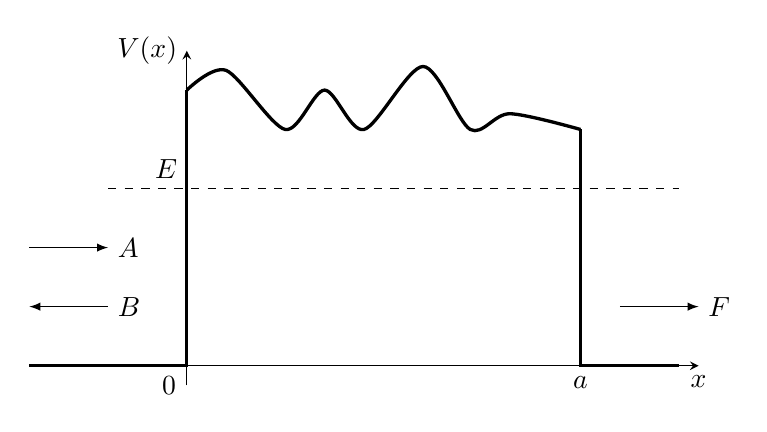
\begin{tikzpicture}
\draw[-stealth] (-0.5,0) -- (6.5,0)node[below]{$x$};
\draw[-stealth] (0,-0.25) -- (0,4)node[left]{$V(x)$};
%\draw[very thick](-2,0) -- (0,0) -- (0,3) to [out=30,in=180] ++(0.5,0) to [out=0,in=180] ++(0.75,-0.25) to [out=0,in=180] +%+(1,0.5) to [out=0,in=180] (5,3.5) -- (5,0)node[below]{$a$}-- (6,0);
\draw[very thick](-2,0) -- (0,0) node[below left]{$0$}-- (0,3.5) (5,3)--(5,0)node[below]{$a$}--(6.25,0);
\draw[very thick] plot [smooth] coordinates {(0,3.5)(0.5,3.75)(1.25,3)(1.75,3.5)(2.25,3)(3,3.8)(3.6,3)(4.1,3.2)(5,3)};
\draw[dashed](-1,2.25)--(6.25,2.25);
\draw[-latex](-2,1.5)--++(1,0)node[right]{$A$};
\draw[latex-](-2,0.75)--++(1,0)node[right]{$B$};
\draw[-latex](5.5,0.75)--++(1,0)node[right]{$F$};
\draw(0,2.25)node[above left]{$E$};
\end{tikzpicture}
\caption{موڑے دار بالائی سطح کی   مستطیلی رکاوٹ سے بکھراو۔}
\label{شکل_وکب_مستطیلی_رکاوٹ}
\end{figure}

ایک مثال کے طور پر،   مستطیلی رکاوٹ جس کی بالائی سطح غیر ہموار ہو (شکل \حوالہ{شکل_وکب_مستطیلی_رکاوٹ}) سے بکھراو کے مسئلے  پر غور کریں۔ رکاوٹ کی بائیں جانب \عددی{(x<0)} 
\begin{align}
	\psi(x)=Ae^{ikx}+Be^{-ikx}
\end{align}
ہو گا، جہاں \عددی{A} آمدی حیطہ اور \عددی{B} منعکس حیطہ ہے،  اور  \عددی{k\equiv\sqrt{2mE}/\hslash} ہے( حصہ \حوالہ{حصہ_غیر_تابع_ڈیلٹا_تفاعل_مخفیہ} دیکھیں)۔ رکاوٹ کے دائیں جانب \عددی{(x>a)}
\begin{align}
	\psi(x)=Fe^{ikx}
\end{align}
ہو گا؛ \عددی{F} ترسیلی حیطہ ہے،   اور  ترسیلی احتمال درج ذیل ہوگا۔
\begin{align}
	T=\frac{\abs{F}^{2}}{\abs{A}^{2}}
\end{align}
سرنگ زنی خطہ \عددی{(0\leq x\leq a)} میں ونٹزل و کرامرس و برلوان  تخمین درج ذیل دیگی۔
\begin{align}
	\psi(x)\cong\frac{C}{\sqrt{\abs{p(x)}}}e^{\frac{1}{\hslash}\int^{x}_{0}| p(x')| \dif x'}+\frac{D}{\sqrt{\abs{p(x)}}}e^{-\frac{1}{\hslash}\int^{x}_{0}| p(x')| \dif x'}
\end{align}

\begin{figure}
\centering
\begin{tikzpicture}
\draw[-stealth] (-2.75,0) -- (6,0)node[below]{$x$};
%\draw[-stealth] (0,-0.25) -- (0,4)node[left]{$V(x)$};
\draw[-stealth](-360/200,0) -- (-360/200,1) node[pos=0.5, fill=white]{$A$};
\draw[thick,domain=-560:0] ({\x/200},{cos(\x)});
\draw[thick,smooth](0,1) to [out = 0,in=160] ++ (1,-0.25) to [out=-20,in=170] ++ (2,-0.55);
\draw[thick,domain=0:900] plot[smooth] ({3+\x/400},{-0.1+0.3*cos(\x)});
\draw[dashed](0,0) -- (0,1.25) (1,1) -- (-2.25,1); 
\draw[](0,0.1)--++(0,-0.2) node[below]{$0$};
\draw[dashed](2.9,0) -- (2.9,0.5) (2.9,0.2) -- (5.25,0.2); 
\draw[](2.9,0.1)--++(0,-0.2) node[below]{$a$};
\draw[-stealth] (3.925,-0.5) -- (3.925,0);
\draw[stealth-] (3.925,0.2) -- (3.925,0.75) node[right]{$F$};
\end{tikzpicture}
\caption{اونچی اور چوڑی رکاوٹ سے بکھراو کے تفاعل  موج کی کیفی ساخت۔}
\label{شکل_وکب_اونچی_چوڑی}
\end{figure}


اگر رکاوٹ بہت بلند، یا  بہت چوڑا  یا دونوں ہو  (یعنی جب سرنگ زنی کا احتمال بہت کم ہو)،  تب  قوت نمائی بڑھتے جزو کا عددی سر \عددی{(C)} لازماً چھوٹا ہوگا ( درحقیقت،\ترچھا{  لامتناہی} چوڑے  رکاوٹ کی صورت میں یہ\ترچھا{ صفر}  ہوگا)،  اور تفاعل موج کا نقش شکل \حوالہ{شکل_وکب_اونچی_چوڑی}  کی طرز\حاشیہد{اس تجسسی دلیل کو زیادہ  پختہ بنایا جا سکتا ہے (سوال \حوالہ{سوال_وقب_پختہ_دلیل} دیکھیں)۔}  کا ہوگا۔ غیر کلاسیکی خطہ پر قوت نمائی میں کل کمی،  آمدی اور ترسیلی امواج کے حیطوں کے تناسب کو   تعین کرتا ہے 
\begin{align*}
	\frac{\abs{F}}{\abs{A}}\sim e^{-\frac{1}{\hslash}\int^{a}_{0}| p(x') |\dif x'}
\end{align*}
 لہٰذا درج ذیل ہوگا۔
\begin{align}\label{مساوات_وقب_ترسیلی_حیطہ}
	T\cong e^{-2\gamma}, \quad    \gamma\equiv\frac{1}{\hslash}\int^{a}_{0}\abs{p(x)}\dif x
\end{align}
\ابتدا{مثال}
\اصطلاح{الفا تحلیل کا نظریہ گامو۔}\فرہنگ{نظریہ گامو!الفا تحلیل}\حاشیہب{Gamow's theory of alpha decay}\فرہنگ{Gamow's theory}  \سن{1928} میں جارج گامو نے مساوات \حوالہ{مساوات_وقب_ترسیلی_حیطہ}   استعمال کرتے ہوئے الفا تحلیل   (    چند مخصوص تابکار مراکزہ سے، دو پروٹان اور دو نیوٹران پر مشتمل،    الفا ذرہ  کے اخراج )کی وجہ پیش کی۔ چونکہ الفا ذرہ مثبت بار \عددی{(2e)} کا حامل ہے،  لہٰذا جیسے ہی یہ  مرکزوی بندشی قوت کی پہنچ سے باہر نکلتا ہے،   باقی مرکزہ  ( کے بار \عددی{(Ze)}کی  برقی    قوت دافع اس کو  دور جانے پر مجبور کرتی  ہے۔ لیکن،  اس کو پہلے اس مخفی رکاوٹ سے گزرنا ہوگا ( جو یورینیم کی صورت میں)  خارجی الفا ذرے  کی توانائی سے دو گنا  سے بھی زیادہ ہے۔ گامو نے اس مخفی توانائی کو تخمینی طور پر  (پروٹان کے رداس)         \عددی{r_1} وسعت  کے  چوکور کنواں  ( جو مرکزوی قوت کشش کو     ظاہر کرتا  ہے)    کو کولمب قوت دافع کی دم سے  جوڑ کر ظاہر  کیا (شکل \حوالہ{شکل_وکب_گامو_نمونہ})،  اور   کوانٹائی سرنگ زنی کو الفا ذرہ کی فرار کی وجہ قرار دیا  ( مرکزوی طبیعیات پر کوانٹائی میکانیات کے  اطلاق کا یہ  پہلا واقع ہے)۔

\begin{figure}
\centering
\begin{tikzpicture}[declare function={f(\x)= 1/(\x);}]
\pgfmathsetmacro{\E}{f(4)}
\begin{axis}[axis lines=middle,xlabel={$r$},ylabel={$V(r)$}, xtick={1,4},
 xticklabels={\rlap{$\, r_1$} ,$r_2$, $0$}, ytick={-0.5,\E}, yticklabels={$-V_0$,$E$}, ylabel style={at={(current axis.above origin)},anchor=east},xlabel style={at={(current axis.right of origin)},anchor=north east},enlargelimits]
\addplot [thick,domain=1:5]{f(x)}node[pos=0.5,pin={45:{\RL{کولمب دفع}}}]{};
\addplot[thick,]coordinates{({1},{f(1)})(1,-0.5)(0,-0.5)};
\addplot[thick,]coordinates{(0,\E)(5,\E)};
\addplot[]coordinates{(0.75,-0.5)}node[pin={45:{\RL{مرکزوی بندش}}}]{};
\end{axis}
\end{tikzpicture}
\caption{تابکار مرکزہ  میں الفا ذرے  کی مخفی توانائی کا گامو نمونہ۔}
\label{شکل_وکب_گامو_نمونہ}
\end{figure}


اگر خارج  الفا ذرے کی توانائی \عددی{E} ہو،   بیرونی واپسیں  نقطے  \عددی{(r_2)}  کا  تعین درج ذیل  کرے گا۔
\begin{align}
	\frac{1}{4\pi\epsilon_{0}}\frac{2Ze^{2}}{r_{2}}=E
\end{align}
ظاہر ہے  قوت نما \عددی{\gamma}  (مساوات \حوالہ{مساوات_وقب_ترسیلی_حیطہ})  درج ذیل ہوگا۔\حاشیہد{یہاں رکاوٹ کی  بائیں جانب مخفیہ صفر نہیں ہے  (مزید،  حقیقتاً یہ تین بعدی مسئلہ ہے)، تاہم   مساوات \حوالہ{مساوات_وقب_ترسیلی_حیطہ} میں پیش بنیادی تصور سے ہمیں  دلچسپی ہے۔}
\begin{align*}
	\gamma=\frac{1}{\hslash}\int^{r_{2}}_{r_{1}}\sqrt{2m\Big(\frac{1}{4\pi\epsilon_{0}}\frac{2Ze^{2}}{r}-E\Big)}\,\dif r=\frac{\sqrt{2mE}}{\hslash}\int^{r_{2}}_{r_{1}}\sqrt{\frac{r_{2}}{r}-1}\,\dif r
\end{align*}
اس تکمل میں \عددی{r\equiv r_2\sin^2u} پُر کرکے  نتیجہ حاصل کرتے ہیں۔
\begin{align}
	\gamma=\frac{\sqrt{2mE}}{\hslash}\left[r_{2}\left(\frac{\pi}{2}-\sin^{-1}\sqrt{\frac{r_{1}}{r_{2}}}\right)-\sqrt{r_{1}(r_{2}-r_{1})}\right]
\end{align}
عام طور پر \عددی{r_1\ll r_2} ہوگا،  لہٰذا ہم چھوٹے زاویوں کا  تخمین \عددی{(\sin\epsilon\cong\epsilon)} استعمال کر کے  اس نتیجے  کا سادہ روپ حاصل کرتے ہیں:
\begin{align}\label{مساوات_وقب_عرصہ_حیات_اصل}
	\gamma\cong\frac{\sqrt{2mE}}{\hslash}\left[\frac{\pi}{2}r_{2}-2\sqrt{r_{1}r_{2}}\right]=K_{1}\frac{Z}{\sqrt{E}}-K_{2}\sqrt{Zr_{1}}
\end{align}
جہاں 
\begin{align}
	K_{1} \equiv \left(\frac{e^{2}}{4\pi\epsilon_{0}}\right)\frac{\pi\sqrt{2m}}{\hslash}= \SI{1.980}{\mega\electronvolt^{1/2}},
\end{align}
اور درج ذیل ہوگا۔
\begin{align}
	K_{2} \equiv \left(\frac{e^{2}}{4\pi\epsilon_{0}}\right)^{1/2}\frac{4\sqrt{m}}{\hslash}= \SI{1.485}{\femto\meter^{-1/2}}.
\end{align}
(عمومی مرکزہ کی جسامت تقریباً \عددی{\SI{e-15}{\meter}} یعنی \عددی{\SI{1}{\femto\meter}}  ہوتی ہے۔)

اگر ہم مرکزہ کے اندر الفا ذرے  کو محصور تصور کریں اور کہیں کہ اسکی اوسط سمتی رفتار \عددی{v} ہے،  تب دیواروں کے ساتھ تصادم کے بیچ اوسط وقفہ تقریباً \عددی{2r_1/v} ہوگا،  لہٰذا تصادم کا تعدد \عددی{v/2r_1} ہوگا۔ ہر تصادم پر فرار ہونے کا احتمال \عددی{e^{-2\gamma}} ہے،  لہٰذا اکائی وقت میں اخراج کا احتمال \عددی{(v/2r_1)e^{-2\gamma}} ہوگا،  اور یوں مائی  مرکزہ کا \اصطلاح{ عرصہ حیات}\فرہنگ{عرصہ حیات}\حاشیہب{lifetime}\فرہنگ{lifetime}  تقریباً درج ذیل ہوگا۔
\begin{align}\label{مساوات_وقب_عرصہ_حیات}
	\tau=\frac{2r_{1}}{v} e^{2\gamma}.
\end{align}
بدقسمتی سے ہم \عددی{v} نہیں جانتے، لیکن اس سے زیادہ فرق نہیں پڑتا،  چونکہ ایک تابکار مرکزہ سے اور دوسرے تابکار مرکزہ کے بیچ قوت  نمائی جزو ضربی پچیس رتبی  تک تبدیل ہوتا ہے؛ اس کے سامنے \عددی{v} کی تبدیلی قابل نظرانداز ہے۔ بالخصوص ، عرصہ حیات کی تجرباتی پیمائشی قیمتوں کو \عددی{1/\sqrt{E}} کے ساتھ ترسیم کرنے سے ایک خوبصورت سیدھا خط  (شکل \حوالہء{8.6})حاصل ہوتا ہے جو عین مساوات \حوالہ{مساوات_وقب_عرصہ_حیات_اصل}  اور مساوات \حوالہ{مساوات_وقب_عرصہ_حیات}  کے تحت ہوگا۔
\انتہا{مثال}
\ابتدا{سوال}
ایک متناہی چوکور رکاوٹ، جس کی اونچائی \عددی{V_0>E} اور چوڑائی \عددی{2a} ہے،  سے  ایسے ذرے،  جس کی توانائی \عددی{E} ہے،  کی تخمینی ترسیمی احتمال  مساوات \حوالہ{مساوات_وقب_عرصہ_حیات}  استعمال کرتے ہوئے حاصل کریں۔ اپنے جواب کا موازنہ  اصل  نتیجے  (سوال \حوالہ{سوال_غیر_تابع_مستطیل_رکاوٹ_چوڑائی_معلوم})  کے ساتھ کریں، جس تک  ونٹزل و کرامرس و برلوان  طریق \عددی{T\ll 1}  میں اس کی تخفیف ہو گی۔
\انتہا{سوال}
\ابتدا{سوال}
مساوات \حوالہ{مساوات_وقب_عرصہ_حیات_اصل}  اور مساوات \حوالہ{مساوات_وقب_عرصہ_حیات}  استعمال کرتے ہوئے \عددی{\ce{U^{238}}} اور \عددی{\ce{Po^{212}}} کے عرصہ حیات تلاش کریں۔ \ترچھا{اشارہ:}تمام    مراکزہ میں مرکزوی مادہ کی کثافت تقریباً  ایک جیسی  ہوتی ہے،  لہٰذا \عددی{(r_1)^3}   (پروٹان اور نیوٹران کی تعداد کے مجموعہ) \عددی{A}   کا راست متناسب ہو گا۔ تجرباتی طور پر درج ذیل حاصل کیا گیا ہے۔
\begin{align}
	r_{1}\cong(\SI{1.07}{\femto\meter})A^{1/3}
\end{align}
خارج شدہ الفا ذرے کی توانائی،  کلیہ آئنشٹائن \عددی{(E=mc^2)} سے اخذ کی جا سکتی ہے
\begin{align}
	E=m_{p}c^{2}-m_{d}c^{2}-m_{\alpha}c^{2}
\end{align}
جہاں \عددی{m_p} مائی مرکزہ کی کمیت،  \عددی{m_d} بیٹی مرکزہ کی کمیت،  اور \عددی{m_\alpha} الفا ذرے ( یعنی \عددی{\ce{He^4}} مرکزہ)  کی کمیت ہے۔ یہ دیکھنے کی خاطر کہ بیٹی مرکزہ کیا ہوگا ، یاد رہے  کہ الفا ذرہ دو پروٹان اور دو نیوٹران لے کر فرار ہوتا ہے،  لہٰذا \عددی{Z} سے دو  اور \عددی{A} سے چار منفی کریں۔ حاصل جوابات استعمال کرتے ہوئے دوری جدول سے کیمیائی عنصر کا  تعین کریں۔ سمتی رفتار \عددی{v} کی اندازاً قیمت \عددی{E=(1/2)m_{\alpha} v^2} سے حاصل کریں؛  یہ مرکزہ کے اندر منفی مخفی توانائی کو نظرانداز کرتی ہے،  لہٰذا \عددی{v} کی قیمت اصل سے زیادہ دیگی،  تاہم اب تک  ہم صرف اتنا ہی کر سکتے ہیں۔ اتفاقی طور پر ان کیمیائی عناصر کی تجربہ سے حاصل کردہ  عرصہ حیات بالترتیب \عددی{6\times10^9} سال اور \عددی{ \SI{0.5}{\micro\second}}  ہے۔
\انتہا{سوال}
%=======================

\حصہ{کلیات   پیوند}
اب تک کے بحث و فکر میں میں فرض کرتا رہا کہ مخفی کنویں ( یا رکاوٹ) کی" دیواریں" \ترچھا{  انتصابی} تھیں،        جس کی بنا پر بیرونی حل آسان اور سرحدی شرائط سادہ تھے۔ درحقیقت،  ہمارے  مرکزی  نتائج  (مساوات \حوالہ{مساوات_وقب_کوانٹازنی_شرط}  اور مساوات \حوالہ{مساوات_وقب_ترسیلی_حیطہ})    اس صورت میں  بھی کافی حد تک درست ثابت ہوتے ہیں  جب کناروں کی ڈھلان   زیادہ نہ ہو  ( یقیناً نظریہ گامو میں ایسی  صورت پر  ہی ان کا اطلاق کیا گیا)۔ بہر حال،   نقطہ واپسیں  \عددی{(E=V)}،  جہاں "کلاسیکی" اور "غیر کلاسیکی" خطے   جڑتے ہیں اور ونٹزل و کرامرس و برلوان  تخمین ناقابل استعمال ہو گی،  پر ہم  تفاعل موج کا قریبی مطالعہ کرنا چاہیں گے۔ اس حصہ میں میں مقید حال مسئلہ  (شکل \حوالہ{شکل_وکب_کلاسیکی_مقید_خطہ})  پر غور کروں گا؛   آپ مسئلہ بکھراو ( سوال \حوالہ{سوال_وقب_پختہ_دلیل}) حل  کریں گے۔\حاشیہد{انتباہ: درج ذیل دلائل زیادہ تکنیکی ہیں جنہیں پہلی مرتبہ پڑھ کر سمجھنا ضروری نہیں۔}
\begin{figure}
\centering
\begin{tikzpicture}
\fill[lgray] (-1,0.5) rectangle (1,3.75);
\draw[-stealth](-3,-0.5) -- (3.5,-0.5) node[below]{$x$};
\draw[-stealth](0,-0.75) -- (0,4) node[left]{$V(x)$};
\draw[] (-2.75,2.125) -- (2.75,2.125) node[right]{$E$};
\draw[name path=a,decoration={random steps,segment length=0.5mm,amplitude=0.5pt},decorate](-1,0.5) -- (-1,3.75);
\draw[name path=b,decoration={random steps,segment length=0.5mm,amplitude=0.5pt},decorate](1,0.5) -- (1,3.75);
\draw[decoration={brace,amplitude=5pt,raise=4pt, mirror,aspect=0.3},decorate] (-1,0.5) -- (1,0.5) node[midway,below left,yshift=-12pt]{\RL{پیوندکار خطہ}};
\draw[](0,2.125) node[pin={[pin distance=1.25cm]135:{\RL{نقطہ واپسیں}}}]{} --++ (45:2) node[pos=1,pin={10:{\RL{خط بند مخفیہ}}}]{};
\draw[](0,2.125) --++ (-135:2);
\draw[thick] (0,2.125) to [out=45,in=180] (2,3);
\draw[thick] (0,2.125) to [out=-135,in=0] (-2,1.25);
\draw[] (-2,-0.75) -- (-0.25,-0.75) node[pos=0.5,below]{\RL{کلاسیکی خطہ}}; 
\draw[] (+2,-0.75) -- (+0.25,-0.75) node[pos=0.5,below]{\RL{غیر کلاسیکی خطہ}}; 
\end{tikzpicture}
\caption{دائیں ہاتھ نقطہ واپسیں کو  وضاحت سے دکھایا گیا ہے۔}
\label{شکل_وکب_نقطہ_واپسیں_وضاحت}
\end{figure}


اپنی آسانی کی خاطر، ہم محدد  یوں  منتخب  کرتے  ہیں کہ دائیں ہاتھ کا نقطہ واپسیں \عددی{x=0} پر واقع ہو (شکل \حوالہ{شکل_وکب_نقطہ_واپسیں_وضاحت})۔ ونٹزل و کرامرس و برلوان  تخمین میں درج ذیل ہوگا۔
\begin{align}\label{مساوات_وقب_تخمین}
	\psi (x) \cong
	\begin{cases}
		\frac{1}{\sqrt{p(x)}}\left[B e^{\frac{i}{h} \int^{0}_{x} p(x^{'}) \dif x^{'}} + C e^{- \frac{i}{h} \int^{0}_{x} p(x^{'}) \dif x^{'}}\right] ,& x < 0 \\
		\frac{1}{\sqrt{\abs{p(x)}}} D e^{- \frac{1}{h} \int^{x}_{0}|p(x^{'})| \dif x^{'}},& x> 0 
	\end{cases}
\end{align}
(یہ فرض کرتے ہوئے  کہ تمام \عددی{x>0} کے لئے  \عددی{E} سے \عددی{V(x)} بڑا ہوگا،  ہم اس خطہ میں مثبت قوت نما کو خارج کر سکتے ہیں،  چونکہ \عددی{x\to\infty} پر  یہ بے قابو بڑھتا ہے۔)  ہمارا کام ان دو حل  کو سرحد پر ایک دوسرے کے ساتھ جوڑنا ہے۔ لیکن  یہاں ہمیں شدید مشکلات کا سامنا در پیش ہے: ونٹزل و کرامرس و برلوان  تخمین میں  نقطہ واپسیں ( جہاں \عددی{p(x)\to0} ہوگا)  پر  \عددی{\psi} کی قیمت لامتناہی تک پہنچتی ہے۔ حقیقی تفاعل موج یقیناً ایسا رویہ نہیں رکھتا؛ جیسا ہمارا گمان تھا،   ونٹزل و کرامرس و برلوان  تخمین نقطہ واپسیں کی پڑوس میں ناقابل استعمال ہے۔ لیکن اجازتی توانائیوں کا تعین  نقاط واپسیں پر سرحدی شرائط  کرتی ہیں۔ ہم ایک ایسا  "پیوندکار" تفاعل موج لیتے ہیں جو نقطہ واپسیں کو ڈھانپ کر دونوں اطراف کے ونٹزل و کرامرس و برلوان  تخمین حل کو ایک دوسرے کے ساتھ پیوند کرتا ہو۔

چونکہ ہمیں پیوندکار تفاعل موج \عددی{(\psi_p)} صرف مبدا کے  پڑوس میں چاہیے،   لہٰذا ہم اس مخفیہ کو سیدھی لکیر: 
\begin{align}\label{مساوات_وقب_خط_بند_مخفیہ}
	V(x) \cong E + V'(0)x,
\end{align}
سے تخمین دے  کر،  اس خط بند  \عددی{V} کے لئے مساوات شروڈنگر:
\begin{align*}
	-\frac{\hslash^{2}}{2m} \frac{\dif^{\,2}\psi_{p}}{\dif x^{2}} +[E+V'(0)x]\psi_{p}=E\psi_{p}
\end{align*}
یا 
\begin{align}
	\frac{\dif^{\,2} \psi_{p}}{\dif x^{2}} = \alpha^{3} x\psi_{p}
\end{align}
 حل کرتے ہیں، جہاں درج ذیل ہے۔
\begin{align}\label{مساوات_وقب_خط_بند_اور_مستقل}
	\alpha\equiv\left[\frac{2m}{\hslash^{2}} V'(0)\right]^{1/3}
\end{align}
درج ذیل متعارف کر کے ہم ان \عددی{\alpha} کو غیر تابع متغیر میں ضم  کر سکتے ہیں
\begin{align}
	z\equiv\alpha x
\end{align}
لہٰذا درج ذیل ہوگا۔
\begin{align}
	\frac{\dif^{\,2}\psi_{p}}{\dif z^{2}}=z\psi_{p}
\end{align}
یہ \اصطلاح{ مساوات ایئری}\فرہنگ{مساوات ایئری}\حاشیہب{Airy's equation}\فرہنگ{Airy's equation}  ہے جس کے حلوں کو \اصطلاح{ تفاعلات ایئری}\فرہنگ{تفاعلات ایئری}\حاشیہب{Airy functions}\فرہنگ{Airy functions} کہتے  ہیں۔ \حاشیہد{کلاسیکی طور پر، خطی مخفیہ سے مراد مستقل قوت، لہٰذا مستقل اسراع ہے؛ یہ  سادہ ترین  حرکت ہے، جہاں سے  بنیادی میکانیات کا آغاز  ہوتا ہے۔ ستم  ظریفی کی بات ہے کہ یہی سادہ مخفیہ، کوانٹائی میکانیات میں  ماورائی تفاعلات کو جنم دیتا ہے، اور اس  نظریہ میں کلیدی کردار ادا نہیں کرتا۔ } چونکہ مساوات ایئری دو رتبی تفرقی مساوات ہے،  لہٰذا دو خطی غیر تابع ایئری تفاعلات \عددی{\Ai(z)} اور \عددی{\Bi(z)} پائے جاتے ہیں۔

\begin{table}[h!]
\centering
\caption{ایئری تفاعلات کے چند خواص۔}
\label{جدول_وقب_ایئری_تفاعلات}
\renewcommand{\arraystretch}{2}
\begin{tabular}{r l}
\toprule
تفرقی مساوات: & $\frac{\dif^{\,2}y}{\dif z^2}=zy$\\
حل: & ایئری تفاعلات \عددی{\Ai(z)} اور \عددی{\Bi(z)}  کے خطی مجموعے۔ \\
تکملی روپ: &
$\Ai(z)=\frac{1}{\pi}\int_{0}^{\infty}\cos\big(\frac{s^3}{3}+sz\big)\dif s$\\ 
&$\Bi(z)=\frac{1}{\pi}\int_{0}^{\infty}\big[e^{-\frac{s^3}{3}+sz}+\sin\big(\frac{s^3}{3}+sz\big)\big]\dif s$\\
متقاربی روپ:\\
{$\left.\begin{aligned}
\Ai(z)&\sim \frac{1}{2\sqrt{\pi}z^{1/4}}e^{-\frac{2}{3}z^{3/2}}\\
\Bi(z)&\sim\frac{1}{\sqrt{\pi}z^{1/4}}e^{\frac{2}{3}z^{3/2}}
\end{aligned}\right\}z\gg 0$}
&
{$\left.\begin{aligned}
\Ai(z)&\sim \frac{1}{\sqrt{\pi}(-z)^{1/4}}\sin\big[\frac{2}{3}(-z)^{3/2}+\frac{\pi}{4}\big]\\
\Bi(z)&\sim\frac{1}{\sqrt{\pi}(-z)^{1/4}}\cos\big[\frac{2}{3}(-z)^{3/2}+\frac{\pi}{4}\big]
\end{aligned}\right\}z\ll 0$}\\
\bottomrule
\end{tabular}
\end{table}

ان کا تعلق رتبہ \عددی{1/3} کے بیسل تفاعلات کے ساتھ ہے؛  ان کے چند خواص جدول \حوالہ{جدول_وقب_ایئری_تفاعلات}  میں پیش کیے گئے ہیں جبکہ شکل  \حوالہء{8.8}  میں انہیں ترسیم کیا گیا ہے۔ ظاہر ہے کہ پیوندکار تفاعل موج \عددی{\Ai(z)} اور \عددی{\Bi(z)} کا خطی جوڑ :
\begin{align}\label{مساوات_وقب_پیوندی_تفاعل_موج}
	\psi_{p}(x) = a\Ai(\alpha x)+ b\Bi(\alpha x)
\end{align}
ہوگا، جہاں \عددی{a} اور \عددی{b} مناسب مستقلات ہیں۔


\begin{figure}
\centering
\begin{tikzpicture}
\fill[lgray] (-2.5,0.5) rectangle (-1.5,3.75);
\fill[lgray] (1.5,0.5) rectangle (2.5,3.75);
\draw[-stealth](-3,0.5) -- (3.5,0.5) node[below]{$x$};
\draw[](0,-0.65) -- (0,4);
\draw[name path=a,decoration={random steps,segment length=0.5mm,amplitude=0.5pt},decorate](-2.5,0.5) -- (-2.5,3.75);
\draw[name path=b,decoration={random steps,segment length=0.5mm,amplitude=0.5pt},decorate](-1.5,0.5) -- (-1.5,3.75);
\draw[name path=a,decoration={random steps,segment length=0.5mm,amplitude=0.5pt},decorate](2.5,0.5) -- (2.5,3.75);
\draw[name path=b,decoration={random steps,segment length=0.5mm,amplitude=0.5pt},decorate](1.5,0.5) -- (1.5,3.75);
\draw[decoration={brace,amplitude=5pt,raise=4pt, mirror},decorate] (-2.5,0.5) -- (-1.5,0.5) node[midway,below,yshift=-12pt]{\RL{منطبق خطہ \عددی{1}}};
\draw[decoration={brace,amplitude=5pt,raise=4pt, mirror},decorate] (1.5,0.5) -- (2.5,0.5) node[midway,below,yshift=-12pt]{\RL{منطبق خطہ \عددی{2}}};
\draw[] (-2.5,-0.75) -- (2.5,-0.75) node[pos=0.5,below]{\RL{پیوندکار خطہ}};
\draw[](0,0.5) node[fill=black,circle,inner sep=1.5pt]{} node[pin={[text centered, text width=1cm]45:{\RL{نقطہ واپسیں}}}]{};
\draw[stealth-stealth] (-2.5,2.5) -- (2.5,2.5) node[pos=0.6,fill=white]{$\psi_p$};
\draw[stealth-] (-1.5,3) -- (-3.75,3) node[above right]{$\psi_{WKB}$};
\draw[stealth-] (1.5,3) -- (3.75,3) node[above left]{$\psi_{WKB}$};
\end{tikzpicture}
\caption{پیوندی خطہ اور دو  منطبق  خطے۔}
\label{شکل_وکب_پیوندکار_منطبق}
\end{figure}

اب \عددی{\psi_p} مبدا کے  پڑوس میں ( تخمینی)  تفاعل موج ہے؛  ہم نے مبدا کے دونوں اطراف   منطبق   خطوں  میں \عددی{\psi_p} کو ونٹزل و کرامرس و برلوان   حلوں کے ساتھ ہم پلہ  بنانا ہوگا ( شکل \حوالہ{شکل_وکب_پیوندکار_منطبق}  دیکھیں)۔ یہ منطبق  خطے  نقاط  واپسیں کے اتنے  قریب ہیں کہ خط بند مخفیہ   کافی  درست ہوگا ( لہٰذا \عددی{\psi_p} اصل تفاعل موج کا بہترین تخمین ہوگا )، اور  ساتھ ہی   نقاط واپسیں  سے اتنے   دور ضرور  ہیں کہ ونٹزل و کرامرس و برلوان  تخمین پر بھروسہ کیا جا سکتا ہے۔\حاشیہد{یہ نازک  دوہری مسلط    شرط ہے،اور ایسے گھمبیر   مخفیے  تیار کرنا  ممکن ہے کہ جن میں اس طرح کا کوئی منطبق خطہ نہ پایا جاتا ہو۔ البتہ، عملی استعمال میں ایسا شاذ و نادر ہی ہوتا ہے۔ سوال \حوالہ{سوال_وقب_شاذونادر} دیکھیں۔  }  منطبق   خطوں میں مساوات \حوالہ{مساوات_وقب_خط_بند_مخفیہ}  کارآمد ہے،  لہٰذا (  مساوات \حوالہ{مساوات_وقب_خط_بند_اور_مستقل}  کی علامتیت  میں)  درج ذیل ہوگا۔
\begin{align}\label{مساوات_وقب_پیوندکار_تفاعل_اب_بھی}
	p(x) \cong \sqrt{2m(E-E-V'(0)x)} =\hslash\alpha^{3/2}\sqrt{-x}
\end{align}
بالخصوص  منطبق  خطہ \عددی{2}   میں
\begin{align*}
	\int^{x}_{0} \abs{p(x')} \dif x' \cong \hslash\alpha^{3/2} \int^{x}_{0}\sqrt{x'}\dif x'=\frac{2}{3}\hslash(\alpha x)^{3/2}
\end{align*}
ہو گا، لہٰذا ونٹزل و کرامرس و برلوان   تفاعل موج (مساوات \حوالہ{مساوات_وقب_تخمین})  درج ذیل لکھی جا سکتی ہے۔
\begin{align}
	\psi(x)\cong\frac{D}{\sqrt{\hslash}\alpha^{3/4}x^{1/4}} e^{-\frac{2}{3}(\alpha x)^{3/2}}
\end{align}
 ایئری تفاعلات کی بڑی \عددی{z}  متقاربی روپ\حاشیہد{پہلی نظر میں،  اس خطہ میں ، جسے  \عددی{z=0} پر نقطہ واپسیں کا قریب تصور کیا گیا ہے  (لہٰذا مخفیہ کا خط بند تخمین کارآمد ہو گا)،  بڑی \عددی{z} تخمین کا استعمال  نامعقول  نظر آتا ہے۔ لیکن یہاں تفاعل کا  دلیل \عددی{z} نہیں  \عددی{\alpha x} ہے، اور اگر آپ غور کریں (سوال \حوالہ{سوال_وقب_شاذونادر} دیکھیں) تو آپ دیکھیں گے  کہ ( عموماً)  ایسا خطہ ہو گا جہاں  \عددی{\alpha x} بڑا ہو گا، اور ساتھ ہی  \عددی{V(x)} کو خطی لکیر سے تخمین دینا   معقول  ہو گا۔}   (جدول \حوالہ{جدول_وقب_ایئری_تفاعلات})  استعمال کرتے ہوئے،    منطبق  خطہ \عددی{2}  میں پیوند کار  تفاعل موج (مساوات \حوالہ{مساوات_وقب_پیوندی_تفاعل_موج}) درج ذیل روپ اختیار کرتی ہے۔
\begin{align}
	\psi_{p}(x)\cong \frac{a}{2\sqrt{\pi}(\alpha x)^{1/4}} e^{-\frac{2}{3}(\alpha x)^{3/2}} +\frac{b}{\sqrt{\pi}(\alpha x)^{1/4}} e^{\frac{2}{3}(\alpha x)^{3/2}}
\end{align}
دونوں حلوں کے موازنہ سے درج ذیل لکھا جا سکتا ہے۔
\begin{align}\label{مساوات_وقب_اے_ڈی}
	a=\sqrt{\frac{4\pi}{\alpha\hslash}}D&& \text{\RL{اور}}&& b=0
\end{align}

ہم یہی کچھ  منطبق  خطہ  \عددی{1}  کے لئے بھی کرتے ہیں۔ اب بھی مساوات \حوالہ{مساوات_وقب_پیوندکار_تفاعل_اب_بھی}  ہمیں \عددی{p(x)} دیگی،  تاہم اس مرتبہ  \عددی{x} \ترچھا{ منفی} ہوگا، لہٰذا
\begin{align}
	\int^{0}_{x} p(x')\dif x' \cong \frac{2}{3}\hslash(-\alpha x)^{3/2}
\end{align}
ہو گا، اور ونٹزل و کرامرس و برلوان   تفاعل موج  (مساوات \حوالہ{مساوات_وقب_تخمین})  درج ذیل ہوگا۔
\begin{align}
	\psi(x)\cong\frac{1}{\sqrt{\hslash}\alpha^{3/4}(-x)^{1/4}} \left[B e^{i\frac{2}{3}(-\alpha x)^{3/2}} + C e^{-i\frac{2}{3}(-\alpha x)^{3/2}}\right]
\end{align}
ساتھ ہی بہت بڑی  \ترچھا{منفی}  \عددی{z} کے لئے ایئری تفاعل کا متقارب روپ  (جدول \حوالہ{جدول_وقب_ایئری_تفاعلات})  استعمال کرتے ہوئے پیوندی تفاعل(مساوات \حوالہ{مساوات_وقب_پیوندی_تفاعل_موج}  جس میں \عددی{b=0} لیا گیا ہو)  درج ذیل ہوگا۔
\begin{align}
	\psi_{p}(x) &\cong\frac{a}{\sqrt{\pi}(-\alpha x)^{1/4}} \sin \left[\frac{2}{3}(-\alpha x)^{3/2}+\frac{\pi}{4}\right]\nonumber \\
	&=\frac{a}{\sqrt{\pi}(-\alpha x)^{1/4}}\frac{1}{2i}\left[e^{i\pi/4} e^{i\frac{2}{3}(-\alpha x)^{3/2} - e^{-i\pi/4} e^{-i\frac{2}{3}(-\alpha x)^{3/2}}} \right]
\end{align}
منطبق  خطہ \عددی{1}  میں ونٹزل و کرامرس و برلوان  اور پیوندی تفاعلات موج کے موازنے سے
\begin{align*}
	\frac{a}{2i\sqrt{\pi}} e^{i\pi/4}=\frac{B}{\sqrt{\hslash\alpha}}&& \text{\RL{اور}}&& \frac{-a}{2i\sqrt{\pi}}e^{-i\pi/4}=\frac{C}{\sqrt{\hslash\alpha}}.
\end{align*}
حاصل ہو گا، جس میں \عددی{a} کی قیمت مساوات  \حوالہ{مساوات_وقب_اے_ڈی}  سے پر کر کے درج ذیل حاصل ہوگا۔
\begin{align}
	B=-ie^{i\pi/4}D&&\text{\RL{اور}}&&C=ie^{-i\pi/4}D
\end{align}
انہیں\اصطلاح{ کلیات جوڑ}\فرہنگ{کلیات جوڑ}\حاشیہب{connection formulas}\فرہنگ{connection formulas}  کہتے ہیں،  جو نقطہ واپسیں کے دونوں اطراف ونٹزل و کرامرس و برلوان   حلوں کو آپس میں  پیوند کرتے ہیں۔ پیوندی تفاعل موج کا کام،  نقطہ واپسیں پر پیدا درز کو ڈھانپنا تھا؛  اس کی ضرورت  آگے  نہیں آئے گی۔تمام  چیزوں کو   معمول زنی مستقل \عددی{D} کی صورت میں بیان کر کے نقطہ واپسیں کو واپس مبدا سے اختیاری نقطہ \عددی{x_2} منتقل کرتے ہوئے،  ونٹزل و کرامرس و برلوان تفاعل موج (مساوات \حوالہ{مساوات_وقب_تخمین}) درج ذیل روپ اختیار کرتا ہے۔
\begin{align}\label{مساوات_وقب_تفاعل_موج_حاصل}
	\psi(x)\cong
	\begin{cases}
		\frac{2D}{\sqrt{p(x)}} \sin\left[\frac{1}{\hslash}\int^{x_{2}}_{x} p(x') \dif x' +\frac{\pi}{4} \right], & x\textless x_{2} \\
		\frac{D}{\sqrt{\abs{p(x)}}} \exp\left[-\frac{1}{\hslash}\int^{x}_{x_{2}} \abs{p(x')}\dif x' \right], & x\textgreater x_{2}
	\end{cases}
\end{align}

\ابتدا{مثال}
\موٹا{ایک انتصابی دیوار والا مخفیہ کنواں۔} فرض کریں ایک مخفیہ کنویں کی \عددی{x=0} پر انتصابی دیوار جبکہ دوسری دیوار ڈھلان  ہے (شکل \حوالہ{شکل_وکب_ایک_دیوار_کنواں})۔ ایسی صورت میں \عددی{\psi(0)=0} ہوگا لہٰذا  مساوات \حوالہ{مساوات_وقب_تفاعل_موج_حاصل}  کے تحت 
\begin{align*}
	\frac{1}{\hslash}\int^{x_{2}}_{0} p(x)\dif x+\frac{\pi}{4}=n\pi,&&(n=1,2,3,\dotsc)
\end{align*}
یا درج ذیل ہوگا۔
\begin{align}\label{مساوات_وقب_کوانٹا_زنی_شرط}
	\int^{x_{2}}_{0}p(x)\dif x=\big(n-\frac{1}{4}\big)\pi\hslash
\end{align}

\begin{figure}
\centering
\begin{tikzpicture}
\fill[path fading=west,color=lgray] (-0.25,0) rectangle (0,3.75);
\draw[-stealth] (-0.5,0) -- (5.75,0)node[below]{$x$};
\draw[-stealth] (0,-0.25) -- (0,4)node[left]{$V(x)$};
\draw[very thick, name path=a] (0,3.5) -- (0,0.25) to [out=0,in=180] ++ (2,1) to [out=0,in=-120] ++ (2,1) to [out=60,in=-160] ++ (1,1); 
\draw[name path=b](0,2) node[left,xshift={-0.5em}]{$E$} -- (5,2);
\draw[dashed,name intersections={of={a and b}}] (intersection-2) -- ($(0,0)!(intersection-2)!(5,0)$) node[below]{$x_2$};
\end{tikzpicture}
\caption{ایک  انتصابی  دیوار والا مخفیہ کنواں۔}
\label{شکل_وکب_ایک_دیوار_کنواں}
\end{figure}

مثلاً،  " نصف ہارمونی مرتعش": 
\begin{align}
	V(x)=
	\begin{cases}
		\frac{1}{2}m\omega^{2}x^{2}, & x> 0 , \\
		0, &\text{\RL{دیگر صورت}}
	\end{cases}
\end{align}
پر غور کریں۔ اس صورت میں
\begin{align*}
	p(x)=\sqrt{2m[E-(1/2)m\omega^{2}x^{2}]}=m\omega\sqrt{x^{2}_{2}-x^{2}}
\end{align*}
ہوگا،  جہاں
\begin{align*}
	x_{2}=\frac{1}{\omega}\sqrt{\frac{2E}{m}}
\end{align*}
نقطہ واپسیں ہے۔  لہٰذا
\begin{align*}
	\int^{x_{2}}_{0} p(x)\dif x=m\omega\int^{x_{2}}_{0}\sqrt{x^{2}_{2}-x^{2}}\dif x=\frac{\pi}{4}m\omega x^{2}_{2}=\frac{\pi E}{2\omega}
\end{align*}
ہو گا، اور کوانٹازنی شرط  (مساوات \حوالہ{مساوات_وقب_کوانٹا_زنی_شرط}) درج ذیل دیگا۔
\begin{align}
	E_{n}=\left(2n-\frac{1}{2}\right)\hslash\omega=\left(\frac{3}{2}, \frac{7}{2}, \frac{11}{2},\dots\right)\hslash\omega
\end{align}
اس مخصوص صورت میں ونٹزل و کرامرس و برلوان  تخمین  اصل  اجازتی توانائیاں دیتی ہے  (جو\ترچھا{ مکمل}  ہارمونی مرتعش کی طاق توانائیاں ہیں؛ سوال \حوالہ{سوال_غیر_تابع_نصف_ہارمونی_اجازتی}  دیکھیں)۔
\انتہا{مثال}
\ابتدا{مثال}
\موٹا{بغیر انتصابی دیواروں کا مخفیہ کنواں۔} اس نقطہ واپسیں پر جہاں مخفیہ کی ڈھلوان اوپر رخ  (شکل \حوالہ{شکل_وکب_بالائی_جانب_نقطہ_واپسیں}-ا) ہو، مساوات \حوالہ{مساوات_وقب_تفاعل_موج_حاصل}   ونٹزل و کرامرس و برلوان تفاعلات موج کو  آپس میں پیوند کرتی ہے۔ نیچے   ڈھلوان نقطہ واپسیں (شکل \حوالہ{شکل_وکب_بالائی_جانب_نقطہ_واپسیں}-ب)  پر یہی دلائل  درج ذیل دیگا   (سوال \حوالہ{سوال_وقب_نیچے_رخ_نقطہ_واپسیں})۔
\begin{align}\label{مساوات_وقب_نیچے_رخ_نقطہ_واپسیں}
	\psi(x)\cong
	\begin{cases}
		\frac{D'}{\sqrt{|p(x)|}} e^{-\frac{1}{\hslash}\int^{x_{1}}_{x} |{p(x')|\dif x'}},&x< x_{1}  \\
		\frac{2D'}{\sqrt{p(x)}} \sin\big[\frac{1}{\hslash}\int^{x}_{x_{1}}p(x')\dif x'+\frac{\pi}{4}\big],&x> x_{1} 
	\end{cases}
\end{align}
%
\begin{figure}
\centering
\begin{subfigure}{0.22\textwidth}
\centering 
\pgfmathsetmacro{\a}{70}
\pgfmathsetmacro{\b}{180-\a}
\begin{tikzpicture}
%\draw[-stealth] (0,0) -- (0.5,0)node[below]{$x$};
%\draw[-stealth] (0,0) -- (0,3)node[left]{$V(x)$};
\draw[] (-1,0) node[left]{$E$} -- (1,0);
\draw[dashed] (0,-1) node[below]{$x_2$} -- (0,1);
\draw[very thick, name path=a] (0,0) to [out=\a,in=-170] ++ (1,1); 
\draw[very thick, name path=a] (0,0) to [out=-\b,in=10] ++ (-1,-1); 
\end{tikzpicture}
\caption{}
\end{subfigure}\hfill
\begin{subfigure}{0.22\textwidth}
\centering 
\pgfmathsetmacro{\a}{70}
\pgfmathsetmacro{\b}{180-\a}
\begin{tikzpicture}
%\draw[-stealth] (0,0) -- (0.5,0)node[below]{$x$};
%\draw[-stealth] (0,0) -- (0,3)node[left]{$V(x)$};
\draw[] (-1,0) node[left]{$E$} -- (1,0);
\draw[dashed] (0,-1) node[below]{$x_1$} -- (0,1);
\draw[very thick, name path=a] (0,0) to [out=-\a,in=170] ++ (1,-1); 
\draw[very thick, name path=a] (0,0) to [out=\b,in=-10] ++ (-1,1); 
\end{tikzpicture}
\caption{}
\end{subfigure}\hfill
\begin{subfigure}{0.45\textwidth}
\centering 
\pgfmathsetmacro{\a}{70}
\pgfmathsetmacro{\b}{180-\a}
\begin{tikzpicture}
\draw[-stealth] (-1.5,-1.5) -- ++(0.5,0)node[below]{$x$};
\draw[-stealth] (-1.5,-1.5) -- ++(0,3)node[below left]{$V(x)$};
\draw[] (-1,0) node[left]{$E$} -- (3,0);
\draw[dashed] (0,-1) node[below]{$x_1$} -- (0,1);
\draw[dashed] (2,-1) node[below]{$x_2$} -- (2,1);
\draw[very thick, name path=a] (0,0) to [out=-\a,in=180] ++ (1,-1); 
\draw[very thick, name path=a] (0,0) to [out=\b,in=-10] ++ (-1,1); 
\draw[very thick, name path=a] (2,0) to [out=-\b,in=0] ++ (-1,-1); 
\draw[very thick, name path=a] (2,0) to [out=\a,in=-170] ++ (1,1); 
\end{tikzpicture}
\caption{}
\end{subfigure}
\caption{بالائی رخ  ڈھلوان اور نیچے رخ  ڈھلوان نقاط واپسیں۔}
\label{شکل_وکب_بالائی_جانب_نقطہ_واپسیں}
\end{figure}
بالخصوص، مخفیہ کنویں (شکل \حوالہ{شکل_وکب_بالائی_جانب_نقطہ_واپسیں}-ج)  کی بات کرتے ہوئے،"  اندرونی"  خطہ \عددی{(x_1<x<x_2)} میں تفاعل موج کو  
\begin{align*}
	\psi(x)\cong\frac{2D}{\sqrt{p(x)}} \sin\theta_{2}(x),&&\theta_{2}(x)\equiv \frac{1}{\hslash}\int^{x_{2}}_{x} p(x')\dif x'+\frac{\pi}{4}
\end{align*}
(مساوات \حوالہ{مساوات_وقب_تفاعل_موج_حاصل} )،   یا درج ذیل لکھا جا سکتا ہے
\begin{align*}
	\psi(x)\cong\frac{-2D'}{\sqrt{p(x)}} \sin\theta_{1}(x),&&\theta_{1}(x)\equiv -\frac{1}{\hslash}\int^{x}_{x_{1}} p(x')\dif x'-\frac{\pi}{4}
\end{align*}
(مساوات \حوالہ{مساوات_وقب_نیچے_رخ_نقطہ_واپسیں})۔ ظاہر ہے، ماسوائے مضرب \عددی{\pi}  کے،\حاشیہد{سائن تفاعلات کے دلیل میں فرق مضرب \عددی{\pi} نہ کے مضرب \عددی{2\pi} ہو گا، چونکہ مجموعی منفی علامت کو  معمول زنی مستقلات \عددی{D} اور \عددی{D'} میں ضم کیا جا سکتا ہے۔}      سائن تفاعلات کے دلیل لازماً برابر ہوں گے:   \عددی{\theta_2=\theta_1+n\pi}،   لہٰذا درج ذیل ہو گا۔
\begin{align}\label{مساوات_وقب_کوانٹازنی_شرط_ڈھلوان_اطراف}
	\int^{x_{2}}_{x_{1}}p(x)\dif x=\big(n-\frac{1}{2}\big)\pi\hslash,\quad n=1,2,3,\dotsc
\end{align}

 یہ کوانٹازنی شرط،   دو  ڈھلوان اطراف کے "عمومی"   مخفیہ کنویں کی اجازتی توانائیوں کو  تعین کرتا ہے۔  دھیان رہے کہ   دو انتصابی دیواروں کے  کلیہ (مساوات \حوالہ{مساوات_وقب_کوانٹازنی_شرط}) یا  ایک انتصابی دیوار کے  کلیہ (مساوات \حوالہ{مساوات_وقب_کوانٹا_زنی_شرط}) اور موجودہ کلیہ (مساوات \حوالہ{مساوات_وقب_کوانٹازنی_شرط_ڈھلوان_اطراف})  میں صرف اس عدد (\عددی{0}، \عددی{1/4} یا \عددی{1/2})  کا فرق ہے جو \عددی{n}  سے منفی ہوتا ہے۔ چونکہ ونٹزل و کرامرس و برلوان  تخمین  (بڑی \عددی{n} کی)  نیم کلاسیکی  طریق میں بہترین کام کرتی ہے، لہٰذا یہ فرق صرف دکھاوے کی حد تک ہے۔ بہر حال یہ نتیجہ انتہائی طاقتور ہے،  جس کو استعمال کر کے،  مساوات شروڈنگر  حل کیے بغیر،  ایک سادہ تکمل کی قیمت حاصل کر کے تخمینی اجازتی توانائیاں معلوم کی جا سکتی ہیں۔ تفاعل موج خود کہیں نہیں نظر آتا۔
\انتہا{مثال}
\ابتدا{سوال}\شناخت{سوال_وقب_ٹپکیاں_کھاتا_گیند}
زمین پر   لچکدار   ٹپکیاں لیتے  ہوئے  (کمیت \عددی{m} کی)  گیند کے کلاسیکی مسئلے کے مماثل کوانٹائی میکانی مسئلے پر غور کریں۔\حاشیہد{یہ ایک مصنوعی مسئلہ نظر آتا ہے؛ درحقیقت،  نیوٹران کے لئے یہ تجربہ سرانجام دیا گیا ہے۔ }
\begin{enumerate}[a.]
\item
 مخفی توانائی کیا ہوگی اس کو زمین سے بلندی \عددی{x} کا  تفاعل لکھیں؟ (منفی \عددی{x} کی صورت میں مخفیہ لامتناہی ہوگا؛  گیند کبھی وہاں  نہیں جا سکتا۔)
\item
 اس مخفیہ کے لئے مساوات شروڈنگر حل کر کے  جواب کو مناسب ایئری تفاعل کے روپ میں لکھیں ( یاد رہے،  بڑی \عددی{z}  پر  \عددی{\Bi(z)} بےقابو بڑھتا ہے،  لہٰذا اس کو  لازماً رد کرنا ہوگا)۔ تفاعل \عددی{\psi(x)} کی معمول زنی کرنے  کی ضرورت نہیں۔
\item
 پہلی چار اجازتی توانائیوں کو تین معنی خیز ہندسوں تک \عددی{g=\SI{9.80}{\meter/\second\squared}} اور \عددی{m=\SI{0.1}{\kilogram}} لے کر حاصل کریں۔
\item
 اس ثقلی میدان میں ایک الیکٹران کی زمینی حال توانائی،  \عددی{\si{\electronvolt}} میں،  کتنی ہوگی؟ اوسطاً یہ الیکٹران زمین سے کتنی بلندی پر ہوگا؟ \ترچھا{اشارہ:} مسئلہ وریل سے \عددی{\langle x\rangle} کا  تعین کریں۔
 \end{enumerate}
\انتہا{سوال}
\ابتدا{سوال}
 ونٹزل و کرامرس و برلوان   تخمین استعمال کرتے ہوئے (سوال \حوالہ{سوال_وقب_ٹپکیاں_کھاتا_گیند}  کی)  ٹپکیاں  کھاتے ہوئے گیند کا تجزیہ کریں۔
\begin{enumerate}[a.]
\item
 اجازتی توانائیوں  \عددی{E_n} کو \عددی{m}، \عددی{g}  اور \عددی{\hslash} کی صورت میں لکھیں۔
\item
 ابسوال \حوالہ{سوال_وقب_ٹپکیاں_کھاتا_گیند}-ج  میں دی گئی مخصوص قیمتوں کو پُر کر کے ونٹزل و کرامرس و برلوان  تخمین کی ابتدائی چار توانائیوں کا "بالکل ٹھیک"  نتائج کے ساتھ موازنہ کریں۔
\item
کوانٹائی عدد \عددی{n} کو  کتنا بڑا ہونا ہوگا کہ گیند اوسطاً زمین سے،مثلاً،  ایک میٹر کی بلندی پر ہو۔
\end{enumerate}
\انتہا{سوال}
\ابتدا{سوال}
ہارمونی مرتعش کی اجازتی توانائیوں کو ونٹزل و کرامرس و برلوان  تخمین سے حاصل کریں۔
\انتہا{سوال}
\ابتدا{سوال}\شناخت{سوال_وقب_شاذونادر}
ہارمونی مرتعش(جس کی زاویائی تعدد \عددی{\omega} ہو ) کی \عددی{n}ویں ساکن حال میں کمیت \عددی{m} کے ایک ذرے پر غور کریں۔
\begin{enumerate}[a.]
\item
 نقطہ واپسیں،  \عددی{x_2}،  تلاش کریں۔
\item
 نقطہ واپسیں سے کتنی بلندی \عددی{(d)} پر خط بند  مخفیہ (مساوات \حوالہ{مساوات_وقب_خط_بند_مخفیہ}   لیکن  نقطہ واپسیں  \عددی{x_2} پر ہو )   میں سہو  \عددی{1\percent} ہو گا؟  یعنی،  اگر 
\begin{align*}
	\frac{V(x_{2}+d)-V_{\text{\RL{خطی}}}(x_{2}+d)}{V(x_{2})}=\num{0.01}
\end{align*}
ہو،تب \عددی{d} کیا ہوگا؟
\item
 جب تک \عددی{z\geq5} ہو \عددی{\Ai(z)} کا متقاربی روپ \عددی{1\percent} تک درست ہوگا۔ جزو -ب  میں حاصل کردہ \عددی{d} کے لئے \عددی{n} کی ایسی سب سے  کم قیمت تلاش کریں کہ \عددی{\alpha d\geq5} ہو۔  (اس  سے بڑی    \عددی{n} کے لئے ایسا  منطبق  خطہ موجود ہوگا جس میں خط بند  مخفیہ \عددی{1\percent} تک درست  اور بڑی \عددی{z} روپ کا ایئری تفاعل  \عددی{1\percent}  درست ہوگا۔)
 \end{enumerate}
\انتہا{سوال}
\ابتدا{سوال}\شناخت{سوال_وقب_نیچے_رخ_نقطہ_واپسیں}
نیچے  ڈھلوان   نقطہ واپسیں کا  پیوندی کلیہ اخذ کر کے مساوات \حوالہ{مساوات_وقب_نیچے_رخ_نقطہ_واپسیں}   کی تصدیق کریں۔
\انتہا{سوال}
\ابتدا{سوال}\شناخت{سوال_وقب_پختہ_دلیل}
مناسب پیوندی کلیات استعمال کر کے ڈھلوان  دیواروں کی رکاوٹ (شکل \حوالہ{شکل_وکب_ڈھلوانی_دیواروں_رکاوٹ}) سے بکھراو کے مسئلہ پر غور کریں۔\ترچھا{ اشارہ:} درج ذیل روپ کے  ونٹزل و کرامرس و برلوان تفاعل موج سے آغاز کریں۔
\begin{align}
	\psi(x)\cong
	\begin{cases}
		\frac{1}{\sqrt{p(x)}}\left[A e^{\frac{i}{\hslash}\int^{x_{1}}_{x}p(x')\dif x'}+B e^{-\frac{i}{\hslash}\int^{x_{1}}_{x}p(x')\dif x'}\right],& (x < x_{1}) \\
		\frac{1}{\sqrt{|p(x)|}}\left[C e^{\frac{1}{\hslash}\int^{x}_{x_{1}}|p(x')|\dif x'}+D e^{-\frac{1}{\hslash}\int^{x}_{x_{1}}|p(x')|\dif x'}\right],& (x_{1}<x <x_{2}) \\
		\frac{1}{\sqrt{p(x)}}\left[F e^{\frac{i}{\hslash}\int^{x}_{x_{2}}p(x')\dif x'}\right],& (x >x_{2})
	\end{cases}
\end{align}
%
\begin{figure}
\centering 
\begin{tikzpicture}
\pgfmathsetmacro{\a}{135}
\pgfmathsetmacro{\b}{180 - \a}
\draw[-stealth] (-3,0) -- (3,0)node[below]{$x$};
\draw[-stealth] (0,-0.25) -- (0,3)node[left]{$V(x)$};
\draw[name path=a] (-3,1.5) node[left]{$E$} -- (3,1.5);
\draw[very thick, name path=b] (-3,0.2) to [out=10,in=-\a] ++ (2,2) to [out=\b, in=0] (0,2.5) to [out=0,in=-180] ++ (0.5,0.25) to [out=0,in=170] (3,0.2);
\draw[dashed,name intersections={of={a and b}}] (intersection-1) -- ($(-3,0)!(intersection-1)!(3,0)$) node[below]{$x_1$}  (intersection-1) --++ (0,0.25);
\draw[dashed,name intersections={of={a and b}}] (intersection-2) -- ($(-3,0)!(intersection-2)!(3,0)$) node[below]{$x_2$}  (intersection-2) --++ (0,0.25);
\end{tikzpicture}
\caption{ڈھلوانی دیواروں والا رکاوٹ۔}
\label{شکل_وکب_ڈھلوانی_دیواروں_رکاوٹ}
\end{figure}
%
کسی صورت \عددی{C=0} \ترچھا{ مت} لیں۔ سرنگ زنی احتمال \عددی{T=\abs{F}^2/\abs{A}^2} کا حساب کریں، اور  دکھائیں کہ بلند اور چوڑی رکاوٹ کی صورت میں آپ کا نتیجہ
مساوات \حوالہ{مساوات_وقب_ترسیلی_حیطہ}  دے گا۔
\انتہا{سوال}




\جزوحصہء{اضافی سوالات برائے باب \حوالہ{باب_وکب_تخمین}}
\ابتدا{سوال}
عمومی قوت نمائی مخفیہ :
\begin{align*}
	V(x)=\alpha\abs{x}^{\nu}
\end{align*}
جہاں \عددی{\nu} ایک مثبت عدد ہے،  کی اجازتی توانائیوں کو ونٹزل و کرامرس و برلوان  تخمین سے تلاش کریں۔ اپنے نتیجہ کو \عددی{\nu=2} جانچیں۔ \ترچھا{ جواب:}\حاشیہد{ہمیشہ کی طرح،  ونٹزل و کرامرس و برلوان   تخمین نیم کلاسیکی (بڑی \عددی{n})  طریق میں سب سے زیادہ درست ثابت ہوتی ہے۔ بالخصوص، مساوات \حوالہ{مساوات_وقب_قوت_نمائی_نتیجہ} زمینی حال (n=1) کے لئے  اتنی اچھی نہیں ہے۔ }
\begin{align}\label{مساوات_وقب_قوت_نمائی_نتیجہ}
	E_{n}=\alpha\left[(n-1/2)\hslash\sqrt{\frac{\pi}{2m\alpha}}\frac{\Gamma\left(\frac{1}{\nu}+\frac{3}{2}\right)}{\Gamma\left(\frac{1}{\nu}+1\right)}\right]^{\left(\frac{2\nu}{\nu+2}\right)}
\end{align}
\انتہا{سوال}
\ابتدا{سوال}
 ونٹزل و کرامرس و برلوان   تخمین استعمال کر کے سوال \حوالہ{سوال_غیر_تابع_غیر_منعکس_مخفیہ}  کے مخفیہ کے لئے مقید حال توانائی تلاش کریں۔ نتیجے کا ٹھیک ٹھیک جواب کے ساتھ موازنہ کریں۔\ترچھا{ جواب:}  \عددی{-[(9/8)-(1/\sqrt{2})]\hslash^2a^2/m}
\انتہا{سوال}
\ابتدا{سوال}
کروی تشاکلی مخفیہ کے لئے ہم رداسی حصے  (مساوات \حوالہ{مساوات_ابعادی_رداسی})  پر ونٹزل و کرامرس و برلوان  تخمین کا اطلاق کر سکتے ہیں۔ مساوات \حوالہ{مساوات_وقب_کوانٹا_زنی_شرط}  کی درج ذیل روپ کو \عددی{l=0} کی صورت میں استعمال کرنا معقول ہوگا \حاشیہد{رداسی مساوات پر  ونٹزل و کرامرس و برلوان  تخمین کا اطلاق چند نازک اور پیچیدہ مسائل پیدا کرتا ہے، جس پر یہاں کوئی بات نہیں کی جائے گی۔}
\begin{align}
	\int^{r_{0}}_{0}p(r)\dif r=(n-1/4)\pi\hslash
\end{align}
جہاں \عددی{r_0} نقطہ واپسیں ہے، ( یعنی ہم \عددی{r=0} کو لامتناہی دیوار تصور کرتے ہیں)۔ اس کلیہ کو زیر استعمال لاتے ہوئے لوگارتھمی مخفیہ :
\begin{align*}
	V(r)=V_{0}\ln(r/a)
\end{align*}
کی اجازتی توانائیوں کی اندازاً قیمت تلاش کریں ( جہاں \عددی{V_0} اور \عددی{a} مستقلات ہیں)۔ صرف \عددی{l=0} کی صورت پر غور کریں۔ دکھائیں کہ سطحوں کے بیچ فاصلوں کا انحصار کمیت پر نہیں ۔\ترچھا{ جزوی جواب:}
\begin{align*}
	E_{n+1}-E_{n}=V_{0}\ln\left(\frac{n+3/4}{n-1/4}\right)
\end{align*}
\انتہا{سوال}
\ابتدا{سوال}
 ونٹزل و کرامرس و برلوان   تخمین کا  درج ذیل روپ
\begin{align}
	\int^{r_{2}}_{r_{1}}p(r)\dif r=(n-1/2)\pi\hslash
\end{align}
استعمال کر کے ہائیڈروجن کی مقید حال توانائیوں کی اندازاً قیمت تلاش کریں۔ موثر  مخفیہ (مساوات \حوالہ{مساوات_تین_ابعادی_موثر_مخفیہ})  میں مرکز گریز جزو شامل کرنا مت بھولیں۔ درج ذیل تکمل مددگار ثابت ہو سکتا ہے۔
\begin{align}
	\int^{b}_{a}\frac{1}{x}\sqrt{(x-a)(b-x)}\dif x=\frac{\pi}{2}(\sqrt{b}-\sqrt{a})^{2}
\end{align}
آپ دیکھیں گے کہ \عددی{n\gg l} اور \عددی{n\gg1/2} کی صورت میں  بوہر سطحیں   حاصل ہوں  گی۔ \ترچھا{ جواب:}
\begin{align}
	E_{nl}\cong\frac{\SI{-13.6}{\electronvolt}}{[n-(1/2)+\sqrt{l(l+1)}]^{2}}
\end{align}
\انتہا{سوال}
%KKK edited till here 7 feb 2022
\ابتدا{سوال}
تشاکلی دوہرا  کنویں  (شکل \حوالہ{شکل_وکب_تشاکلی_دہرا_کنواں})  پر غور کریں۔ ہم \عددی{E<V(0)} والی مقید حالات میں دلچسپی رکھتے ہیں۔
\begin{figure}
\centering 
\begin{tikzpicture}
\pgfmathsetmacro{\a}{135}
\pgfmathsetmacro{\b}{180 - \a}
\draw[-stealth] (-3,0) -- (3.5,0)node[below]{$x$};
\draw[-stealth] (0,-0.25) -- (0,3)node[left]{$V(x)$};
\draw[name path=a] (-3,1) node[left]{$E$} -- (3,1);
\draw[very thick, name path=b] (0,1.5) to [out=0,in=180] (1,0) to [out=0, in=-100] (3,2.5)  (0,1.5) to [out=180,in=0] (-1,0) to [out=180, in=-90] (-3,2.5);
\draw[dashed,name intersections={of={a and b}}] (intersection-1) -- ($(-3,0)!(intersection-1)!(3,0)$) node[below]{$x_1$}  (intersection-1) --++ (0,0.25);
\draw[dashed,name intersections={of={a and b}}] (intersection-2) -- ($(-3,0)!(intersection-2)!(3,0)$) node[below]{$x_2$}  (intersection-2) --++ (0,0.25);
\end{tikzpicture}
\caption{تشاکلی دہرا کنواں؛ سوال \حوالہء{8.15}۔}
\label{شکل_وکب_تشاکلی_دہرا_کنواں}
\end{figure}


(الف) خطہ (i) \عددی{x>x_2}، (ii) \عددی{x_1<x<x_2} اور (iii) \عددی{0<x<x_1} کے لئے  ونٹزل و کرامرس و برلوان تفاعلات موج لکھیں۔ نقطہ \عددی{x_1} اور \عددی{x_2} پر مناسب پیوندی کلیات کا اطلاق کر کے \حوالہء{مساوات \num{8.46}} میں \عددی{x_2} کے لئے ایسا کیا گیا ہے آپ کو \عددی{x_1} کے لئے کرنا ہوگا درج ذیل دکھائیں
\begin{align*}
	\psi(x)\cong
	\begin{cases}
		\frac{D}{\sqrt{\abs{p(x)}}} \exp\left[-\frac{1}{\hslash}\int^{x}_{x_{2}}\abs{p(x')}\dif x'\right],& (i) \\
		\frac{2D}{\sqrt{p(x)}} \sin\left[\frac{1}{\hslash}\int^{x_{2}}_{x}p(x')\dif x'+\frac{\pi}{4}\right],& (ii) \\
		\frac{D}{\sqrt{\abs{p(x)}}}\left[2 \cos\theta e^{\frac{1}{\hslash}\int^{x_{1}}_{x}\abs{p(x')}\dif x'} +\sin\theta e^{-\frac{1}{\hslash}\int^{x_{1}}_{x}\abs{p(x')}\dif x'}\right],& (iii)
	\end{cases}
\end{align*}
جہاں درج ذیل ہوگا
\begin{align}
	\theta\equiv\frac{1}{\hslash}\int^{x_{2}}_{x_{1}}p(x)\dif  x.
\end{align}
(ب) چونکہ \عددی{V(x)} تشاکلی ہے لہٰذا ہمیں صرف جفت \عددی{(+)} اور طاق \عددی{(-)} تفاعلات موج پر غور کرنا ہوگا۔ اول الذکر صورت میں \عددی{\psi'(0)=0} ہوگا جبکہ موخر الذکر صورت میں \عددی{\psi(0)=0} ہوگا۔ دکھائیں کہ اس سے درج ذیل کوانٹازنی شرط حاصل ہوتی ہے
\begin{align}
	\tan\theta=\pm 2e^{\phi}.
\end{align}
جہاں درج ذیل ہوگا
\begin{align}
	\phi\equiv\frac{1}{\hslash}\int^{x_{1}}_{-x_{1}}\abs{p(x')}\dif x'.
\end{align}
\حوالہء{مساوات \num{8.59}} تخمینی اجازتی توانائیاں تعین کرتی ہے چونکہ \عددی{x_1} اور \عددی{x_2} میں \عددی{E} کی قیمت داخل ہوتی ہے لہٰذا \عددی{\theta} اور \عددی{\phi} دونوں \عددی{E} کے تفاعلات ہوں گے۔

(ج) ہم بالخصوص بلند یا/اور چوڑے درمیانے رکاوٹ میں دلچسپی رکھتے ہیں ایسی صورت میں \عددی{\phi} بڑا ہوگا لہٰذا \عددی{e^\phi} انتہائی بڑا ہوگا۔ ایسی صورت میں \حوالہء{مساوات \num{8.59}} کے تحت \عددی{\theta} کی قیمتیں \عددی{\pi} کی نصف عدد صحیح مضرب کے بہت قریب ہوں گی اس کو ذہن میں رکھتے ہوئے \عددی{\theta=(n+1/2)\pi+\epsilon} جہاں \عددی{\abs{\epsilon}\ll1} ہے لکھ کر دکھائیں کہ کوانٹازنی شرط درج ذیل روپ اختیار کرتی ہے
\begin{align}
	\theta\cong\left(n+\frac{1}{2}\right)\pi\mp\frac{1}{2}e^{-\phi}.
\end{align}
(د) فرض کریں ان میں سے ہر ایک کنواں قطع مکافی ہے
\begin{align}
	V(x)=
	\begin{cases}
		\frac{1}{2}m\omega^{2}(x+a)^{2},& x\textless 0, \text{\RL{اگر}} \\
		\frac{1}{2}m\omega^{2}(x-a)^{2},& x\textgreater 0, \text{\RL{اگر}}
	\end{cases}
\end{align}
اس مخفیہ کو ترسیم کر کے \عددی{\theta} \حوالہء{مساوات \num{8.58}} تلاش کریں اور درج ذیل دکھائیں 
\begin{align}
	E^{\pm}_{n}\cong\left(n+\frac{1}{2}\right)\hslash\omega\mp\frac{\hslash\omega}{2\pi} e^{-\phi}.
\end{align}
تبصرہ: اگر درمیانی رکاوٹ ناقابلِ گزر ہو \عددی{\phi\to\infty} تب ہمارے پاس دو الگ الگ ہارمونی مرتعشات ہوتے اور توانائیاں \عددی{E_n=(n+1/2)\hslash\omega} دوہری انحطاطی ہوتیں چونکہ ذرہ بائیں کنویں میں یا دائیں کنویں میں ہو سکتا ہے۔ متناہی رکاوٹ کی صورت میں دونوں کنویں کے بیچ  رابطہ  ممکن ہوگا لہٰذا انحطاط ختم ہوگا۔ جفت حالات \عددی{(\psi^+_n)} کی توانائی معمولی کم اور طاق تفاعلات \عددی{(\psi^-_n)} کی توانائی معمولی زیادہ ہوگی۔

(و) فرض کریں ذرہ دائیں کنویں سے آغاز کرتا ہے یا یہ کہنا زیادہ درست ہوگا کہ ذرہ ابتدائی طور پر درج ذیل روپ میں پایا جاتا ہے 
\begin{align*}
	\Psi(x,0)=\frac{1}{\sqrt{2}}(\psi^{+}_{n}+\psi^{-}_{n}).
\end{align*}
جن میں حیطوں کی وہ قیمتیں منتخب کی جائیں گی کہ اس کا بیشتر حصہ دائیں کنویں میں پایا جاتا ہو۔ دکھائیں کہ یہ ذرہ ایک کنویں سے دوسرے  اور دوسرے سے واپس پہلا کنویں درج ذیل دوری عرصہ کے ساتھ ارتعاش کرتا رہے گا
\begin{align}
	\tau=\frac{2\pi^{2}}{\omega} e^{\phi}.
\end{align}
(ھ) متغیر \عددی{\phi} کی قیمت جزو (د) میں دی گئی مخصوص مخفیہ کے لئے تلاش کریں اور دکھائیں جب \عددی{V(0)\gg E} ہو تب \عددی{\phi\sim m\omega a^2/\hslash} ہوگا۔
\انتہا{سوال}
\ابتدا{سوال}
\موٹا{شٹارک اثر میں سرنگ زنی۔} بیرونی برقی میدان چالو کرنے سے اصولی طور پر ایک الیکٹران جوہر سے سرنگ زنی کے ذریعے باہر نکل کر جوہر کو بارداریہ بنا سکتا ہے۔ سوال: کیا ایک عمومی شٹارک اثر کے تجربہ میں ایسا ہوگا؟ ہم ایک سادہ ترین یہ بُعدی نمونہ استعمال کر کے احتمال کی اندازاً قیمت دریافت کر سکتے ہیں۔ فرض کریں ایک ذرہ ایک بہت گہری متناہی چوکور کنواں \حوالہء{حصہ \num{2.6}} میں پایا جاتا ہے۔

(الف) کنویں کی تہہ سے زمینی حال توانائی کتنی بلند ہوگی یہاں فرض کریں \عددی{V_0\gg\hslash^2/ma^2} ہے۔ اشارہ: یہ \عددی{2a} چوڑائی کی لامتناہی چوکور کنویں کی زمینی حال توانائی ہے۔

(ب) اب اضطراب \عددی{H'=-\alpha x} متعارف کریں بیرونی برقی میدان \عددی{E=-E_{ext}\ai} میں \عددی{\alpha=eE_{ext}} ہوگا۔ فرض کریں یہ ایک بہت کمزور اضطراب ہے \عددی{(\alpha a\ll\hslash^2/ma^2)}۔ کل مخفیہ کا خاکہ ترسیم کر کے دیکھیں کہ ذرہ اب مثبت \عددی{x} رخ سرنگ زنی کے ذریعے خارج ہو سکتا ہے۔

(ج) سرنگ زنی جزو ضربی \عددی{\gamma} \حوالہء{مساوات \num{8.22}} کا حساب کریں اور ذرے کو فرار ہونے کے لئے درکار وقت کی اندازاً قیمت \حوالہء{مساوات \num{8.28}} معلوم کریں۔ جواب: \عددی{\gamma=\sqrt{8mV^3_0}/3\alpha\hslash, \tau=(8ma^2/\pi\hslash)e^{2\gamma}}۔

(د) معقول اعداد \عددی{V_0=\SI{20}{\electronvolt}} بیرونی الیکٹران کی بندشی توانائی کی عمومی قیمت \عددی{a=\SI{e-10}{\meter}} عمومی جوہر کا رداس \عددی{E_{\text{\RL{بیرونی}}}=\SI{7e6}{\volt/\meter}} تجربہ گاہ میں مضبوط میدان \عددی{e} اور \عددی{m} الیکٹران کا بار اور کمیت لیں۔ عرصہ \عددی{\tau} کا حساب کر کے اس کا موازنہ کائنات کی عمر کے ساتھ کریں۔
\انتہا{سوال}
\ابتدا{سوال}
رہائشی درجہ حرارت پر میز پر ایک کھڑی بوتل کوانٹائی سرنگ زنی کی وجہ سے کتنی دیر میں خود با خود گر سکتی ہے؟ اشارہ: بوتل کو کمیت \عددی{m} رداس \عددی{R} اور قد \عددی{h} کا نلکی تصور کریں۔ گرتی ہوئی بوتل کے وسطی نقطے کا توازنی مقام \عددی{(h/2)} سے بلندی کو \عددی{x} سے ظاہر کریں۔ مخفی توانائی \عددی{mgx} ہوگی اور بوتل اُس صورت گرے گی جب \عددی{x} کی قیمت فاصل قیمت \عددی{x_0=\sqrt{R^2+(h/2)^2}-h/2} تک پہنچے۔ سرنگ زنی احتمال \حوالہء{مساوات \num{8.22}} کو \عددی{E=0} کے لئے حاصل کریں۔ حراری توانائی \عددی{((1/2)mv^2=(1/2)k_BT)} لیتے ہوئے رفتار کی اندازاً 	قیمت \حوالہء{مساوات \num{8.28}} سے معلوم کریں۔ مناسب قیمتیں پُر کر کے اپنا جواب سالوں میں دیں۔
\انتہا{سوال}

